\documentclass[a4paper,10pt]{article}

\title{Serveur domotique}

\author{TERRIE Corentin \\ CROS Bastien \\ MONNIER Matthias}

\date{\today}

\usepackage[utf8]{inputenc}
\usepackage[french]{babel} 
\frenchbsetup{StandardLists=true} % à inclure si on utilise \usepackage[french]{babel}
\usepackage{lmodern} % Pour changer le pack de police
\usepackage{makeidx}
\usepackage{fancyhdr}
\usepackage{graphicx}
\usepackage[lofdepth,lotdepth]{subfig}
\usepackage{float}
\usepackage{hyperref}					% lien hypertext		 
\usepackage[lofdepth,lotdepth]{subfig}	% sous-figure -> permet d'afficher 2 images côte à côte
\usepackage{caption}
%\usepackage{subcaption}
%---------------------------------------------------------
\usepackage{listings}
\usepackage{textcomp}
% JAVA en couleur ;-)- -----------------------------------
%\lstset{
%language=Java,
%basicstyle=\normalsize, % ou ça==> basicstyle=\scriptsize,
%upquote=true,
%aboveskip={1.5\baselineskip},
%columns=fullflexible,
%showstringspaces=false,
%extendedchars=true,
%breaklines=true,
%showtabs=false,
%showspaces=false,
%showstringspaces=false,
%identifierstyle=\ttfamily,
%keywordstyle=\color[rgb]{0,0,1},
%commentstyle=\color[rgb]{0.133,0.545,0.133},
%stringstyle=\color[rgb]{0.627,0.126,0.941},
%}
%----------------------------------------------------------
%\graphicspath{{images/}{/home/img/}}
%\DeclareGraphicsExtensions{.png ,.jpg}

\renewcommand{\labelitemii}{$\bullet$}

\begin{document}
\makeatletter
  \begin{titlepage}
  \centering
      {\Large \textsc{École Universitaire Polytechnique de Montpellier}}\\
      \textsc{Microélectronique et Automatique - Électronique et Informatique Industrielle }\\
    \noindent\hrulefill 
    \\
    \vspace{2 cm}
      {\large	\@date\\}
    \vspace{2cm}
       {\huge \textbf{\@title}} \\
	
	\vspace{1cm}
      
\includegraphics[scale=0.15]{head.png}\\

    \vspace{2em}
        {\large \@author} \\
    
    \vspace{2.6cm}
        
\includegraphics[height=0.15\textheight]{mea.jpg}
        \hfill
        
\includegraphics[height=0.15\textheight]{um.png}
  \end{titlepage}
\makeatother
\tableofcontents
\clearpage

%-------------------------------------------------------------------------------------------------------------

\section{Presentation Projet}

%-- TITE INTRO --
\begin{figure}[H]
\centering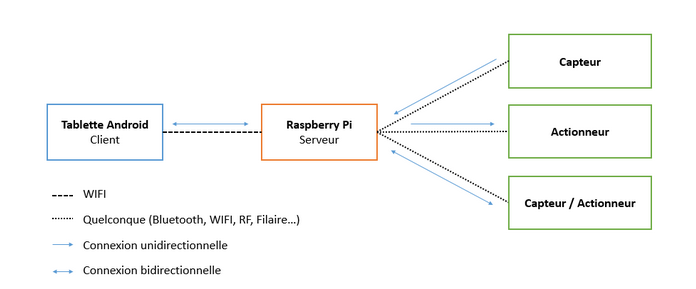
\includegraphics[scale=0.7]{images/Shema_projet.png}
\caption{Schéma montrant les différentes connexion du réseau.}
\end{figure}

%-------------------------------------------------------------------------------

\section{Partie Android (client)}
\subsection{La démarche}
L’application devait seulement servir de client. Cependant, devant la difficulté de débugger et de communiquer entre un client Android et un serveur implémenté sur Raspberry il nous a semblé important de le tester séparément c’est pourquoi nous avons aussi mis en place un serveur Android afin de tester la communication entre deux entités similaires et ainsi s’affranchir des problèmes que peuvent poser deux architectures physiques différentes.  
\subsection{Le client Android}
\subsubsection{Le Socket}
Pour pouvoir communiquer grâce au protocole sélectionné l’application doit prendre en compte plusieurs caractéristiques :
\begin{itemize}
	\item L’adresse IP
	\item Le numéro de port
\end{itemize}
Pour ce faire, on rentre les caractéristiques dans ce qu’on appelle des sockets : il s’agit d’interface de connexion. C’est-à-dire que c’est « l’objet » qui va contenir les informations permettant de se connecter au serveur. L’Android étant un langage de haut niveau proche du Java. Lorsque l’on créer un socket c’est directement lui qui va se charger de faire les bonnes requêtes au serveur et se connecter à celui-ci. Il faut cependant penser à déclarer un code d’erreur permettant de tracer celle-ci en cas d’échec de la connexion. Même si cette étape n’est pas obligatoire elle est vivement conseillée dans le cadre de l’élaboration d’un code professionnel.
\subsection{Le serveur Android}
L’implémentation d’un serveur est peu différente d’un client. Il suffit pour ça de créer un socket serveur dans lequel on va renseigner un numéro de port auquel le client pourra se connecter. Il faut juste vérifier que le numéro de port n’est pas déjà attribué à une autre fonction de l’entité sur lequel on implémente le serveur.

\subsubsection{Le processus}
Le problème lorsque l’on réalise une connexion/communication client/serveur dans une application Android c’est que l’on est obligé de faire tourner cette tâche comme tâche de fond.  En effet, il faut que l’on puisse continuer à utiliser l’application sans que l’on soit déconnecté dès que l’on effectue une nouvelle action. Pour ce faire, il existe plusieurs méthodes pour implémenter un tel comportement. Cependant nous nous préoccuperons seulement des threads ici puisque c‘est la méthode implémentée ici. Lorsqu’une activité est lancée, elle est exécutée dans un thread. Il a pour rôle d’écouter les évènements quand l’utilisateur interagit avec l’interface graphique. Le nom du thread principal est thread UI (interface utilisateur). L’une des règles de programmation est notamment le fait qu’il ne faut pas gérer l’accès à un réseau dans le thread UI. En effet, on ne doit jamais bloquer le thread UI. Or si la connexion échoue, c’est toute l’application qui sera plantée. D’où l’importance de déclarer notre socket dans un nouveau thread. Pour cela, il suffit de déclarer un nouveau thread au sein de notre activité et d’insérer le socket à l’intérieur.
\subsection{Le JSON en Android}
Le langage Android est un langage modulaire donc si l'on veut utiliser le JSON il suffit d’importer le package JSON au début de l’activité dans laquelle on souhaite l’utiliser. On créer ensuite un objet JSON. Pour lui ajouter un nouveau sous-objet, on utilise la fonction puts (syntaxe: objet.puts(1,2)). Le premier paramètre de puts correspond à l’intitulé du second paramètre. Le second paramètre peut quant à lui être : int, double, string… Une implémentation propre d’un objet JSON passe aussi par l’ajout de sa valeur d’erreur afin de tracer celle-ci.
\subsection{L’envoi et la réception de données}
Pour pouvoir envoyer et recevoir des informations il faut créer deux Objects distincts: l’un pour envoyer et l’autre pour recevoir. Ensuite, il suffit d’utiliser une méthode pour recevoir les informations depuis le socket et inversement pour en envoyer. Il y a cependant une subtilité lorsque l’on envoie un objet JSON. En effet, il s’agit d’un objet composé de string. Pour pouvoir réussir à envoyer correctement un message en JSON il faut donc envoyer un Object sur le Stream grâce à la fonction writeObject(). Cependant, il faut convertir cet Object en string sinon le serveur ne sera pas en mesure d’interpréter les données reçues.
\subsection{Le design} 
Afin de créer un environnement pratique pour l’utilisateur, nous avons réalisé une interface comprenant plusieurs onglets :
\begin{itemize}
	\item L’onglet comportant les différents outils de connexions.
	\item L’onglet qui affichera les différentes données issues de la métrologie.
	\item L’onglet permettant de récupérer les différentes informations issues des capteurs et de les contrôler.
\end{itemize}
\begin{figure}[H]
\centering\includegraphics[scale=0.7]{images/page.png}
\caption{Ecran d'acceuil}
\end{figure}
\begin{figure}[H]
\centering\includegraphics[scale=0.7]{images/connexion.png}
\caption{Onglet de connexion}
\end{figure}
\begin{figure}[H]
\centering\includegraphics[scale=0.7]{images/data.png}
\caption{Onglet d'affichage des données}
\end{figure}
\begin{figure}[H]
\centering\includegraphics[scale=0.7]{images/metro.png}
\caption{Onglet de metrologie}
\end{figure}

Les onglets ont une implémentation légèrement plus complexe que le seul appel de différentes activités cependant une fois implémenté leur fonctionnement est similaire. En effet, lorsque l’utilisateur sélectionne l'un des onglets une sous-activité référentes est appelée et l’interface graphique est automatiquement générée grâce au fichier XML associé. Le design en lui-même n’est autre qu’un agencement de widgets et de calques dont les positions sont relatives entre eux afin que l’application s’adapte au mieux à toutes les tailles d’écran. Notre application est cependant optimisée pour des écrans de type tablette (environ 10 pouces).






%-------------------------------------------------------------------------------------------------------------

\section{Partie Raspberry (serveur)}

Le serveur servira a centralisé tout le réseau domotique. Il aura pour tâches : \\
\begin{itemize}
	\item Possibilité de stocker les donnés des capteurs si liaison Tablette-Rasberry coupée.
	\item Gestion des données différentes en fonction de la connexion à un client Android ou un capteur/	actionneur. 
	\item Si connexion à un Android : 
		\begin{itemize}
			\item Envoie des informations concernant les capteurs, les actionneurs, la métrologie.
			\item Réception des ordres de la tablette : allumer tel lampe, se connecter à tel capteur, mettre en action les actionneurs.
		\end{itemize}
	\item Si connexion à un capteur, simplement lire les informations.
	\item Si connexion à un actionneur, le commander (selon les ordres reçu de la tablette) et gérer son état.
	\item Calcul de métrologie pour chaque connexion.
\end{itemize}

Pour implémenter le serveur, nous avons choisi d'utiliser une Raspberry B+, embarquant un système dérivé de Débian : Raspbian. Cela nous as permit d'implémenter un serveur Linux, utilisant les fonctions Unix.

\subsection{Première version du serveur : Connexion à un seul client}

Le premier serveur implémenté sur la Raspberry permettais seulement de gérer une connexion client/serveur la plus simple possible : le client se connecte sur le port du serveur (ici 8888) et grâce à l'adresse IP du serveur à celui-ci, et le serveur notifie sur le terminal que la connexion à bien été effectué. Ensuite le client demande à l'utilisateur de taper un message à l'écran, que le serveur lui renvoi. Finalement le client affiche dans son terminal la réponse du serveur ce qui permet de vérifier que le serveur à bien reçu le message.

\paragraph{Connexion au client Linux}
%% -> les résultats obtenu, qlq images du terminale, puis les prob rencontré ( problème de buffer)

Le premier test à été effectuer en implémentant un client Linux sur la Raspberry. Ainsi, nous pouvions valider le serveur grâce au client, avant de tester la connexion avec le client Android.

Les premiers résultats ont été concluant en terme de connexion, c'est à dire que le serveur reçois la demande de connexion du client et renvois le message du client. Le client, quant à lui, reçois et affiche le message renvoyé par le serveur. Cela nous a permis de valider la création du serveur et la connexion au client. Par contre, nous avons rencontré un problème au niveau du buffer avec le client. En effet, le message affiché à l'écran étais bien celui initialement envoyé, mais le client affiche aussi tous les caractères présent dans le buffer.

\begin{figure}[h]
  \begin{center}
    \subfloat[Connexion au client.]{
      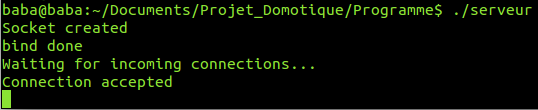
\includegraphics[width=0.5\textwidth]{images/serveur_simple_ex.png}
      \label{sub:serveur_simple}
                         }
    \subfloat[Le client affiche la réponse du serveur.]{
      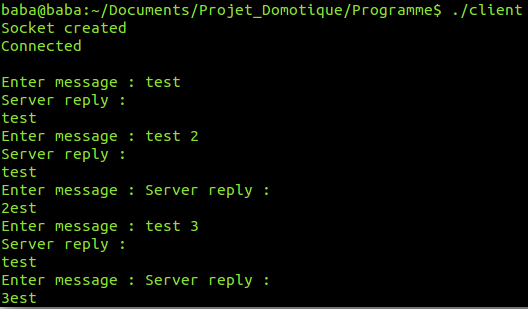
\includegraphics[width=0.5\textwidth]{images/test_reponse_client_simple.png}
      \label{sub:serveur_simple_reponse}
                         }
    \caption{Serveur Linux}
    \label{fig:serv_simple}
  \end{center}
\end{figure}

Comme solution nous avons pensé à gérer la longueur du buffer en fonction de la longueur du message reçu. Mais c'est une autre solution qui a été retenu : un parser. Nous avons choisi le parser JSON, que nous détaillerons plus loin.
%% Faire des test sur cette solution %%


\paragraph{Connexion avec le client Android}
%% -> les résultats obtenu, qlq images du terminale, puis les prob rencontré ( données pas codé de la même manière)
Ensuite il a fallu tester cette solution avec le client sous Android : la conexion a bien marché, mais nous avons eu un premier problème au moment de recevoir le message sur le périphérique Android.

\subsection{Seconde version du serveur : gestion de plusieurs clients}
La deuxième version du serveur nous permet de gérer plusieurs clients à la fois. En effet, de part l'idée du projet, il nous fallait pouvoir gérer plusieurs client, d'origine différente. Pour cela, le serveur appelle un nouveau thread a chaque demande de connexion. Le thread ainsi créé s'exécute ainsi durant la connexion au client. La connexion est quitté si le client arrête de communiquer. 

\paragraph{Connexion au client Linux}
Comme précédemment, nous avons d'abord testé notre programme sur Linux avant Android. La connexion marchais très bien, hormis le problème mentionné dans la première version du serveur. Ce qui est normal car nous n'avons pas encore implémenter le parser.

\paragraph{Connexion avec le client Android}
Le serveur a bien accepté la connexion au client Android, mais nous n'arrivons pas décoder proprement les trames que nous envoyais celui-ci.

\subsection{Troisième version du serveur : échanges de trame au format JSON}

Pour pouvoir parser/déparser nos trames, nous avons choisi d'utiliser  le format de trames JSON. Il présente plusieurs avantage, dont les principaux sont sont son coté générique et abstraits d'une part. Il est donc facilement implémentable sur un langage C (serveur) et JAVA (client). De plus, des parsers existe à la fois sous Linux et Android et ce format de donnée et facilement lisible. Il se presente sous la forme suivante :
\begin{figure}[H]
\centering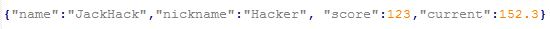
\includegraphics[scale=0.7]{images/JSON_trame.jpg}
%\caption{Schéma montrant les différentes connexion du réseau.}
\end{figure}

Nous avons choisi le parser suivant : \href{https://bitbucket.org/zserge/jsmn/wiki/Home}{parser JSON jsmn}, qui a l'avantage d'être facilement adaptable avec notre programme. Un parser JSON est nativement implémenter dans le système Android, ce qui nous a permis directement tester la communication Android-Linux. \\ 
Le périphérique Android envoie une trame JSON (comme présenté plus haut) et le serveur la décode et l'affiche : 
\begin{figure}[H]
\centering\includegraphics[scale=0.7]{images/test_JSON_litle.jpg}
%\caption{Schéma montrant les différentes connexion du réseau.}
\end{figure}

Le parser jsmn, qui marchait très bien pour une communication Linux-Linux, pose des problèmes dans ce cas ici. En effet, des caractères (ici $"tD"$) sont parsé avant d'arriver à la trame au bon format. La solution envisagée est de coder une fonction qui prends le string reçu qu'a partir de la première accolade.



\subsection{Quatrième version du serveur : lancement de tâche différentes selon le type de connexion}

La version précédentes permettant de gérer plusieurs clients, mais pas de trier la fonction de ceux-ci. Nous avons donc envisagé plusieurs solutions pour résoudre le problème. 

\subparagraph{Différents ports} Au moment de créer le serveur, plusieurs ports sont ouvert. Ainsi, chaque périphérique se connecte au numéro de port correspondant au service requis. Ensuite, le serveur lance le thread correspondant.

\subparagraph{Un identifiant dans la trame JSON} Comme il est facile de modifié les trames sous ce format, il est possible de rajouter un champ pour indiquer quel est le service demandé. 

\subparagraph{Un message comme identifiant} Le premier message de la connexion peut servir à donner l'identifiant du périphérique.

%-------------------------------------------------------------------------------------------------------------

\section{Protocoles domotiques}

\subsection{Les protocoles grand public}
%-----
\paragraph{X10}
Le X10 est un vieux protocole (développé en 1975) par courant porteurs.  Les modules X10 peuvent être piloté par des télécommandes radio (433MHz). 

%\underline{\textbf{Les plus :}}
\subparagraph{Les plus :}
\begin{itemize}
\item Protocole le moins cher dans le domaine des automatismes résidentiels
\item Communauté d'utilisateurs très active
\item Bonne distribution des produits
\end{itemize}
\subparagraph{Les moins :}
\begin{itemize}
\item Gros problème de sécurité (toute personne possédant l'accès à une partie de l'installation électrique peut envoyer des ordres X10)
\item Incompatibilité entre les réseaux électriques des différents pays
\item Pas de retour d'état des modules et collisions non gérées
\end{itemize}
Le X10 est vieillissant et par conséquent de nombres constructeurs le délaissent. Il comporte comme seul avantage d'être simple et n'est donc plus conseillé.
%-----
\paragraph{OREGON}
\paragraph{OREGON}


%-------------
\subsection{Les protocoles de rupture technologique}
Deux protocoles seront détaillés dans cette partie : Z-Wave et EnOcean. Ils partagent de nombreuses similitudes, ils sont tous deux :
\begin{itemize}
\item des protocoles domotiques
\item des technologies sans fil
\item des technologies disponibles via plusieurs centrales domotiques
\item des technologies mises en œuvre par plusieurs constructeurs de périphériques.

\end{itemize}
%-----
\paragraph{Z-Wave}
Le Z-Wave est un protocole radio conçu pour la domotique. Il utilise la fréquence $848.42$MHz.
Ses caractéristiques sont qu'il est relativement sécurisé, à double sens (chaque composant est à la fois récepteur et émetteur) et qu'il utilise un réseau maillé.
%\underline{\textbf{Les plus :}}
\subparagraph{Les plus :}
\begin{itemize}
\item Grande richesse fonctionnelle.
\item Topologie maillée du réseau sans fil (contrainte de portée levée car les périphériques relayent les informations entre eux).
\item Retour d'état des périphérique (acquittement de commande, retour d'état de la batterie etc...).
\item Grande liberté de choix sur les périphériques.
\end{itemize}
\subparagraph{Les moins :}
\begin{itemize}
\item Complexité de la mise en place.
\item Prix élevé des modules.
\item Consommateur de pile.\newline
\end{itemize}
Le Z-Wave est un protocole de choix pour les actionneurs mais moins pour les capteurs. Voici le résumé graphique :

%\begin{figure}[H]
%\centering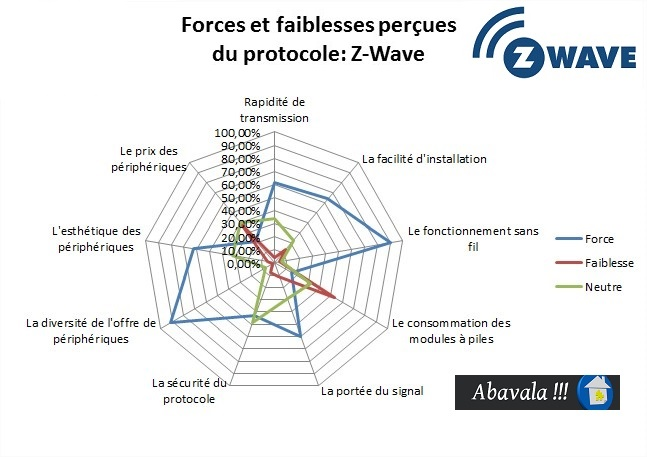
\includegraphics[scale=0.7]{images/forces-protocole-zwave.jpg}
%\caption{Forces et faiblesses du protocole Z-Wave.}
%\end{figure}

%-----
\paragraph{EnOcean}
Le Enocean est également un protocole radio utilisant la fréquence $848.42$MHz. Ce protocole à l'avantage d'être sans fils et sans piles. En effet les périphériques puisent leur source d'énergie de leur environnement direct. Il utilise notamment l'effet photovoltaïque (transforme la lumière en électricité), l'effet piezo-électrique (transforme un choc ou une forte pression en électricité) ainsi que l’effet Peltier ou effet thermoélectrique (transforme une différence de température constaté à un instant donné en électricité).

Lorsqu’un interrupteur EnOcean utilise des cristaux piezo-électrique pour produire son électricité, il communique son ordre ON/OFF par voie hertzienne en utilisant l’énergie fournie par la pression mécanique de celui qui actionne l’interrupteur. Il peut ainsi générer le peu de courant nécessaire pour envoyer l’information à la centrale.

%\underline{\textbf{Les plus :}}
\subparagraph{Les plus :}
\begin{itemize}
\item Flexibilité élevée lors de la mise en oeuvre mais également en cas de modification de l'installation.
\item Pas besoin de changer les piles.
\item Pas de coût de consommables.
\end{itemize}
\subparagraph{Les moins :}
\begin{itemize}
\item Coût des modules plus important que certaines autres technologies.
\item Design peut attrayant de certains modules.
\item Retour d'état non disponible pour certains périphériques (seuls ceux ayant une batterie de stockage de l'énergie le peuvent).
\item Le réseaux n'est pas maillé. Mais il existe des relayeurs graces auxquels le réseaux peut rayonner sur une portée de 200m.\newline
\end{itemize}


Voici le résumé graphique :
%\begin{figure}[H]
%\centering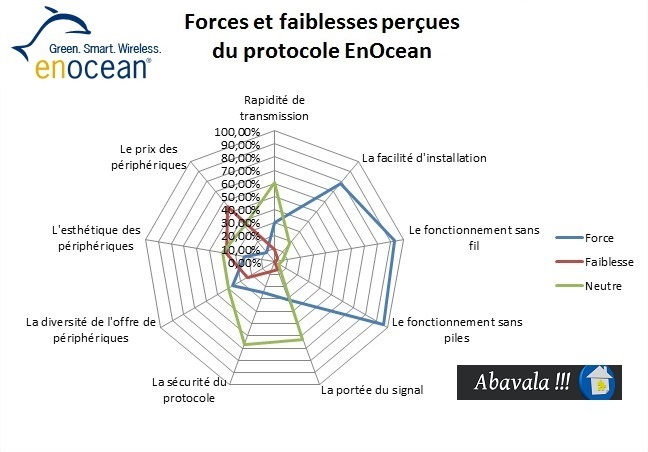
\includegraphics[scale=0.7]{images/forces-protocole-enocean.jpg}
%\caption{Forces et faiblesses du protocole EnOcean.}
%\end{figure}

Les deux graphiques précédent sont issues du site \url{www.abavala.com}. Elles ne sont pas issues de mesures scientifiques mais d’avis personnels exprimés librement. Voici le graphique qui regroupes ces deux protocoles :

%\begin{figure}[H]
%\centering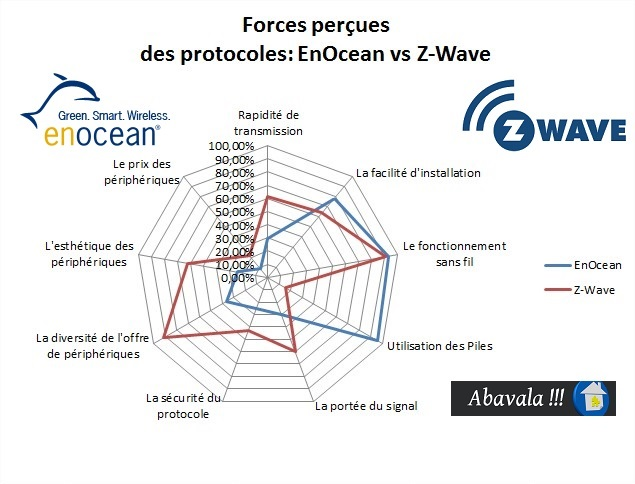
\includegraphics[scale=0.7]{images/forces-enocean-vs-z-wave.jpg}
%\caption{Comparaison des deux protocoles.}
%\end{figure}
%-------------------------------------------------------------------------------------------------------------

\section{Annexes}


 
%-------------------------------------------------------------------------------------------------------------

\end{document}
